\chapter{Systems}
\thispagestyle{fancy}
\minitoc[n] % Creating an actual minitoc

\section{Introduction}


\section{Airframe}
The airframe is aluminium alloy construction except for steel components comprising the engine mount, main
landing gear mounts, control bellcranks and other miscellaneous items. Fibreglass mouldings are used for the
tips of wings and tail surface as well as for the engine cowls, wheel spats and empennage fairings.
The aircraft is conventionally configured with a non laminar flow aerofoil; the effect of surface irregularities is
relatively minor compared to a laminar flow aerofoil.

\section{Engine and propeller}
The aircraft is powered by a LYCOMING IO-360-A1B6 four cylinder, direct drive, horizontally opposed, air cooled, fuel injected engine rated at 200 HP at 2700 rpm. 

The engine is fitted with a 60-amp 14-volt alternator,
Sky Tec starter, high-pressure fuel pump and dual magneto ignition system. 

The induction air filter is mounted in
a ram air snorkel in the left air intake. An alternate air door is mounted to the side of the air snorkel for emergency
use should the induction intake or filter be blocked.

The exhaust system is all-stainless Vetterman four into two configuration and no mufflers. A heat shroud provides cabin
heat as required being ducted to the centre section of the firewall.

Please refer to the Lycoming Operators Handbook for detailed information on maintenance, care and operation
of the engine.

\section{Landing gear}
In conventional configuration the landing gear legs are of spring steel (6150).%, to which a preformed stiffener has been fitted to the front of main legs to improve dampening. 
The tail wheel is steerable and additional steering is possible through differential braking.

The main gear wheels are fitted with Cleveland wheels and disc brakes. The braking system consists of toe
brakes attached to the rudder pedals operating individual Cleveland brake cylinders to each of the main landing
wheels.
These share a common reservoir installed on the top right front face of the fire wall. The brake fluid used is MIL-
H-5606 and is red in colour.

\section{Flying controls}
Flight control integrity is essential for safe flight. At installation or after maintenance it should be confirmed that
ALL controls are connected, secured and safe tied and that they all operate within the specified ranges
smoothly and in the correct direction. Full travel should be confirmed prior to each flight. NO play should be
permitted in the control hinges; sloppiness may induce flutter. Similarly trim tabs must be free of play.

Dual controls are provided. Elevator and Ailerons are operated through a system of adjustable pushrods. The
rudder is operated through a cable system to the rudder pedals. 

An electric elevator and aileron trim system
enables operation of the elevator trim tab and aileron spring bias system.
The elevator and aileron trims can be operated from a rocker switch on the instrument panel. 

\section{Engine controls}
Engine controls consist of a throttle control, pitch control, mixture control,
cabin heat and an alternate air control, mounted at centre beneath the avionics panel.

The throttle (black) is used to adjust engine power output, forward being full throttle and rearward for idle. A
throttle friction nut is located at the base of the control.

The propeller pitch control (blue) is located between the throttle and mixture control. Forward is full fine and
rearwards coarse. The control is of the vernier type and can be operated by rotating the blue knob clockwise or
anti clockwise for small adjustments or by pressing the centre knob in and pushing or pulling the control in or
out.

The mixture control (red) is used to adjust the fuel to air ratio. The engine is shut down by placing the mixture
control in the idle cut-off, or rearward position. The control is of the vernier type and can be operated by rotating
the red knob clockwise or anti clockwise for small adjustments or by pressing the centre knob in and pushing or
pulling the control in or out.

%The cabin heat is used to operate a door on the exhaust heat shroud . To activate, the ratchet cable and knob must be pulled to open the hot air inlet.

The alternate air is used to operate a sliding door on the side of the induction box. To activate, the ratchet cable
and knob must be pulled to open the door. This allows the engine to obtain warm unfiltered air from within the
cowling area. This control should only be used when an induction filter or intake blockage is suspected. Once
operated the control should be manually reset following rectification of the induction system blockage.

\section{Fuel System}
Fuel is stored in two 21 US gal (20 US gal usable) tanks secured to the leading edge structure with screws and
plate nuts. Fuel drains are fitted to the lowest point of each tank (and of the fuel system) and should be drained
prior to the first flight of the day to check for sediment and water.

Two fuel tank vents are located under the main fuselage on the left and rights side just forward of the main
landing gear attachments. These should be checked for any blockages.

The fuel selector valve is located in the centre column. It has four selectable positions - left or right tank and two
fuel shut-off positions.

An auxiliary electric fuel boost pump is fitted forward of the fuel selector on the cabin side of the fire wall and is
used in case of engine driven pump failure and is also used %during take off and landing, and 
when changing fuel
tanks in flight. A switch marked FUEL PUMP is located on the instrument panel.

%An airframe fuel filter is located in the gascolator on the right side of the engine firewall. This filter element
%should be inspected at least every 100hrs or Annual whichever comes first. Shorter cleaning intervals should be
%adopted should fuel quality be questionable.
Two fuel quantity indicators form part of the EFIS display and receive a signal from capacitive type fuel
probes mounted in the fuel tanks. Both are marked to indicate the appropriate fuel tank. These indicators only
register from a set quantity and NOT from full. As with all fuel gauges, these will tend to be inaccurate
when flight attitude is not coordinated or level and during turbulence.

A FUEL FLOW indicator and TOTAL FUEL QTY readout form part of the EFIS display and obtains fuel flow information
from a sender unit mounted in the main fuel line between the fuel selector and the engine driven fuel pump. This
should be used as a more accurate way of determining fuel consumption and fuel remaining. This system relies
on the pilot accurately loading the current fuel quantity into the EFIS whenever fuel is added.

\section{Electrical System}
A block diagram of the aircraft electrical system is provided in Figure~\ref{fig:electrical}.

\begin{sidewaysfigure}
\begin{figure}[H]
\centering
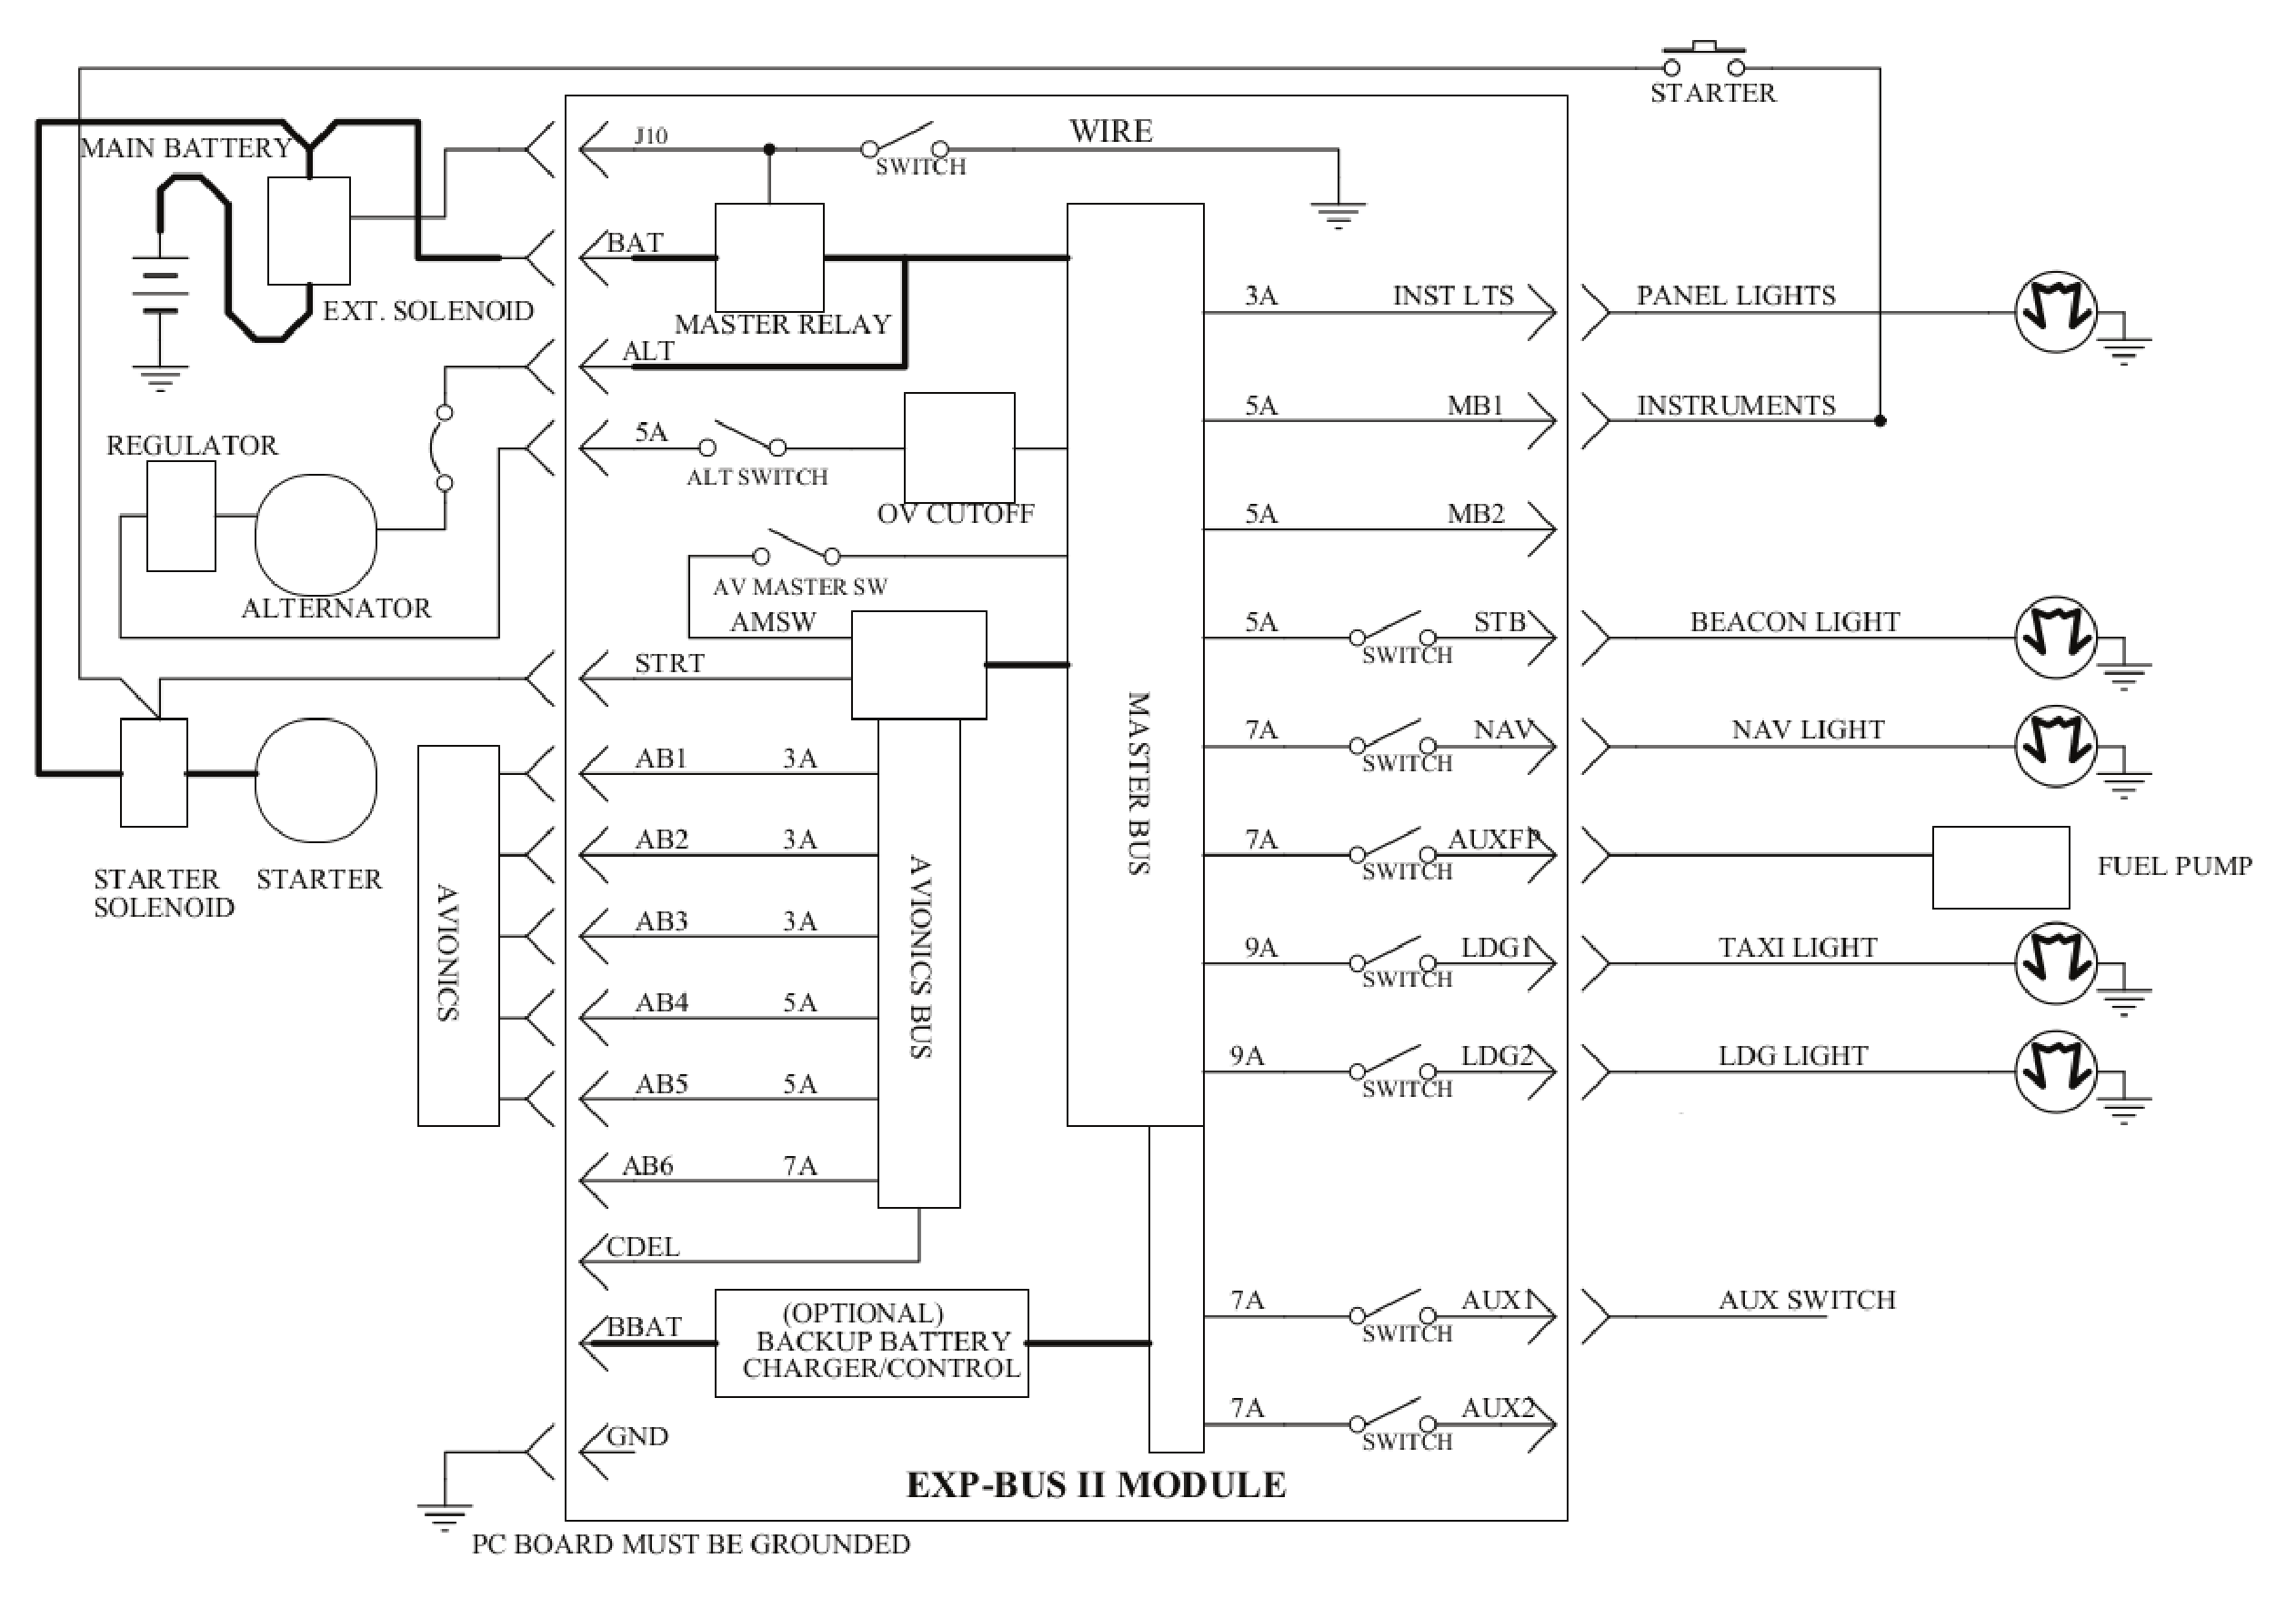
\includegraphics[height=0.6\textheight]{elec_block.eps}
\caption{Electrical system block diagram}
\label{fig:electrical}
\end{figure}
\end{sidewaysfigure}

The electrical system includes a 14 volt 60 amp alternator with an internal regulator and overvoltage protection.

The alternator is protected from overload by a 60A fuse mounted on the engine firewall. The main aircraft battery
is a 12-volt sealed Odyssey battery, which is mounted on the right side of the forward firewall just above the
main battery and starter relays.

The aircraft has no conventional circuit breakers but is instead fitted with an EXP BUS DC load centre which
makes use of solid state current limiting devices known as PTC current limiters. These devices have unique
advantages over fuses and circuit breakers. 

Like a fuse, the PTC device 'blows' when too much current is drawn by an offending circuit, however, like a circuit breaker, the PTC can be reset and in fact does this automatically once the load is COMPLETELY removed.

To reset a circuit simply switch the item off and wait about ten to fifteen seconds for the PTC to reset. Should the
fault have cleared, the circuit will be restored when the switch is turned back on.

The alternator field switch is located next to the master switch. This switch will be disabled should the bus voltage exceed 18V.

Electrical accessories include starter, electric fuel pump, flap actuator, exterior lights, trim motors and avionics
as listed in the equipment section.

\section{Instruments}
The aircraft is fitted with a MGL Odyssey EFIS system as its Primary Flight Display and Engine
Management System. The EFIS unit is powered from a dedicated power switch on the instrument panel.  

A system backup battery is mounted behind the EFIS display and is able to hold configuration data only.  

The MGL RDAC engine module is mounted forward of the firewall under the engine cowl and provides the interface between the EFIS and the engine. 

The MGL ADAHRS is mounted in front of the fuel selector switch on top of the fuel pump cover.  
The MGL magnetometer is mounted behind the baggage area bulkhead.  

Outside Air Temperature is obtained from a sensor mounted on the left bottom cockpit behind the pilot rudder pedals.

A standby analogue airspeed indicator and altimeter are fitted for redundancy.

\section{Avionics}
The following aircraft avionics is fitted and powered once the avionics switch is on:
\begin{itemize}
\item The GARMIN GX 327 is a mode C transponder.
\item MGL V6 COM radio
\item Microair COM radio
\end{itemize}

A GPS antenna is mounted on top of the engine mount underneath the top engine cowl.  

\section{Heating and Ventilation}
Cabin heat is provided via a heat muff attached to the exhaust system and fed with high-pressure air from the front
right engine baffle plate. Flow of hot air enters through a valve on the lower centre and is controlled with a
ratchet cable and knob marked CABIN HEAT. Flow is off in the forward position. When in the OFF position, air
passing through the muff and ducts is dumped into the low-pressure section of the cowl.

Fresh air from naca ducts on the forward side of the fuselage is fed into vents on either side of the instrument
panel for front occupants.


\subsection{Canopy and cabin features}
The canopy is unlatched using the handle on the top middle of the canopy.  To open the canopy should be rolled back while lifting the back slightly to ease it up on the guide rail.  

Entry into the cabin is made by first stepping on the wing, taking care not to step onto the flaps.  The area on the wing where it is safe to stand is covered in black non-slip \textit{wingwalk} material.  From the wing step onto the seat over the cabin side and then slide down into a seated position.

The pilot and passenger backrest may be adjusted forward and aft by means of a piano hinge style system.  The backrest may also be angled to more than one position. 

Both seats are fitted with a four-point harness, which should be carefully fitted and adjusted prior to take off. In single person operations the unused straps should be used to secure the seat cushions and to prevent the straps flying about.
Straps should be checked regularly for damage.

\subsection{Baggage space and entry dimensions}
The baggage area is located behind the passenger seat backrests.  The baggage area has a maximum load capacity of 100 lbs and volume of 12 cubic feet.  

 Baggage needs to be lifted over the seatbacks and fit under the rolled back canopy.  This will constrain the maximum dimension of any item in the baggage area.

